\documentclass[a4paper,11pt]{article}
\usepackage{graphicx}
\usepackage{booktabs}
\usepackage{setspace}
\usepackage{parskip}
\onehalfspacing
\begin{document}

\author{Hiromasa Okada}
\title{\vspace{-2cm}Report for Sheet 2\\
\small{Lab Course Machine Learning and Data Analysis}}
\maketitle

\section*{Implementation comments}

In second exercise I have implemented K-means Clustering, hierarchichal agglomerative clustering, ploting dendrogram of this, probability density function and EM algorithm for Gaussian Mixture Models. We use dataset with nxd (n is number of data points and d is the dimension of a data point)
and k means the number of clusters. 

K-means cluster function inputs dataset, a number of clusters and optionaly number of max iteration. And it outputs cluster sets(kx2), the n-dimensional vector r(1xn) of cluster membership and loss function.

Hierarchichal agglomerative clustering function gets a dataset and the vector r to merge cliuseters. Then it returns merge index, R matrix which contains the cluster membership before each agglomeration step and a vector kmloss which contains the loss function value after each agglomeration step. And dendrogram function plots a dendrogram from this informations.

The probability density function is based on mixture of gaussian. It needs dataset, mean point set(kxd) and covariance matrix(kxdxd) as input and returns propability. EM algorithm function calls this function durling the E-step and it initializes mean point set and covariance matrix at the first time.
The EM algorithm function approximates mean points and covariance matrixs after iterations of E-step and M-step

\begin{verbatim}



\end{verbatim}


\section*{Assignment 1}
After the simple implementation it happend that no menbership was in a cluster. The cluster which has no member did not move any more. To avoid this situation I made the cluster will be initialised again in such a case with a following code.

\begin{verbatim}
mu[zero] = (np.var(X,axis=0)**(1/2))*np.random.randn(len(zero),d)+ np.mean(X,axis=0)
\end{verbatim}

This mean only the cluster with no member will be initialized.

\section*{Assignment 4}
\subsection*{Inv or Solve}

If we find an inverse of matrix there are two usuful functions "numpy.linalg.inv" or "numpy.linalg.solve". But which is better to use? By the following test I found the solve is much faster than inv. So I decided to use solve to find the inverse of matrix.

\begin{verbatim}
C = np.random.rand(k,d,d)​

t1 = time.time()
np.linalg.inv(C)
t2 = time.time()​

t3 = time.time()
np.linalg.solve(C,np.ones((k,1,1))*np.eye(d))
t4 = time.time()​

print ("numpy.linalg.inv(): %f sec." % (t2 - t1))
print ("numpy.linalg.solve(): %f sec." % (t4 - t3))


numpy.linalg.inv(): 0.002217 sec.
numpy.linalg.solve(): 0.000724 sec.
\end{verbatim}

\subsection*{Singular case of covariance matrix}
To find the inverse matrix it is important that the matrix is regular. Otherwise the matrix is singular and not to be inversed. If $\det(A)=0$ is satisfied the matrix A is singular. Is there any case that covariance matrix is singular?
the equation of covariance matrix is $C = \frac{1}{n}(X-\mu)(X-\mu)^{T}$. If we have detaset and mean point like following 

\begin{eqnarray*}
X=
\left(
\begin{array}{cccc}
2 & 4 & 6 \\
8 & 10 & 12  
\end{array}
\right)
, \:\:\:\:
\mu = 
\left(
\begin{array}{cccc}
4  \\
10  
\end{array}
\right) 
\end{eqnarray*}
\begin{eqnarray*}
C &=&
\left(
\begin{array}{cccc}
-2 & 0 & 2 \\
-2 & 0 & 2  
\end{array}
\right) 
\left(
\begin{array}{cccc}
-2 & -2\\
0 & 0 \\
2 & 2  
\end{array}
\right) 
= 
\left(
\begin{array}{cccc}
8 & 8\\
8 & 8 \\  
\end{array}
\right) \\
&\Rightarrow& \det(C) =0
\end{eqnarray*}
So in this case the covariance matrix is singular. If a covariance matrix singular is we have to fix it to be a regular matrix. The simple method is that we add small numbers to diagonal of covariance so too make it to be regular but also this doesn't effect the computation of the inverse. For example,
\begin{eqnarray*}
C' &=& C +
\left(
\begin{array}{cccc}
0.001 & 0\\
0 & 0.001 \\  
\end{array}
\right) \\
&=&
\left(
\begin{array}{cccc}
8 & 8\\
8 & 8 \\  
\end{array}
\right) 
+
\left(
\begin{array}{cccc}
0.001 & 0\\
0 & 0.001 \\  
\end{array}
\right) \\
&=&
\left(
\begin{array}{cccc}
8.001 & 8\\
8 & 8.001 \\  
\end{array}
\right) \\
&\Rightarrow & \det(C') \neq 0
\end{eqnarray*}

\begin{verbatim}


\end{verbatim}

\section*{Assignment 5}
\subsection*{Possibility of too small clusters}

If clusters which are near by each other are choosen and the another is far from them, the two clusters will be too small compare to the another cluster. In this case $\gamma$ for clusters which are close to each other will be very small. Number of membership of cluster k is defined by sum of each nth element of $\gamma$ in. Therefore if $\gamma$ is small, the cluster becomes small.

\begin{eqnarray*}
\gamma_{nk} \leftarrow \frac{\hat{\pi_k}g(X_{n};\hat{\mu_{k}},\hat{\Sigma_{k}})}{\sum^{K}_{k'=1}\hat{\pi_{k'}}g(X_{n};\hat{\mu_{k'}},\hat{\Sigma_{k'}})}
\end{eqnarray*}

If $\gamma_k$ for k th cluster is too small, the number of member of k th cluster will be so small that it is almost 0. This case is equivalent to degenerate clusters in K-means.

\section*{Assignment 7}

\subsection*{1.Convergence on local optima}
By both K-means and GMM Convergence on local optima are observed(by K-means it was more often). To get convergence on global optima I had to try several times because whether the global optima is choosen is depend on the first random initialisation of clustérs. When most of initial clusters are close to each other and few are far from them, it is differcult to find global optima. To avoid them at the initial step random choice of clusters shuld be repeated until each cluster has similar distance between each other. 

\subsection*{2.Reliably on finding clusters by each method}

To find the reliability I ploted 10 times by each method.
First is by K-mean and 6 of thems(in 1,3,6,7,8 and 9th plot) have placed cluster points very well. Therfore reliability is simply 60 percent and it is more than 50 percent but the probability that clusters will be miss placed still high. Therefore if we use K-means method, we need to iterate several times to insure.

\begin{figure}[htbp]
  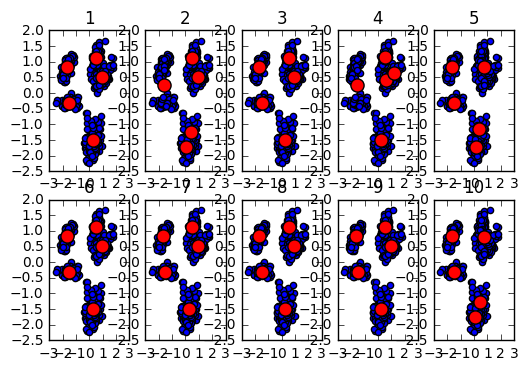
\includegraphics[scale=0.5]{kmean.png}
  \caption{10 times plot with k=5 by K-means}
\end{figure}

By the EM-Algorithm reliability is much higher. In 9 plots of them clusters are placed very well.

Compare to k-means GMM is better at finding global optima. The false placement of cluster by K-means are mostly because of finding local optima. But GMM gets still occasionally chose a local optima, so we need also iteration for GMM.

\begin{figure}[htbp]
  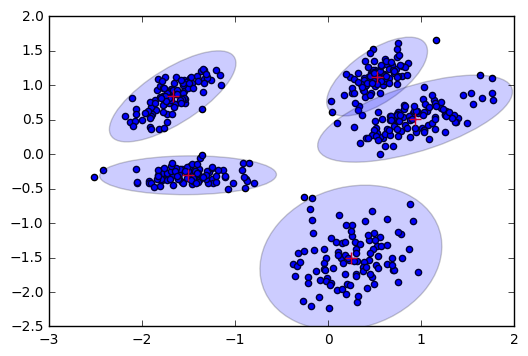
\includegraphics[scale=0.17]{em1.png}
  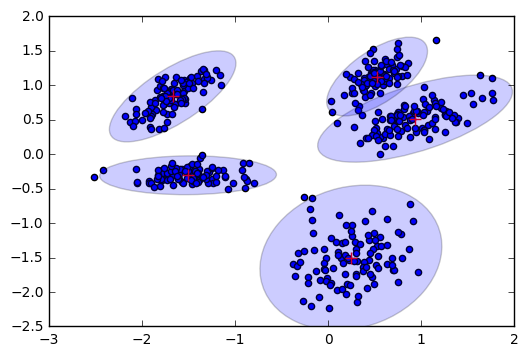
\includegraphics[scale=0.17]{em2.png}
  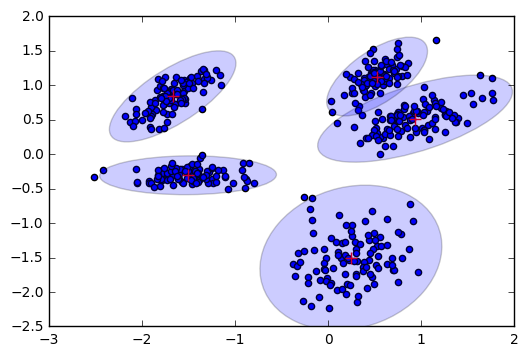
\includegraphics[scale=0.17]{em3.png}
  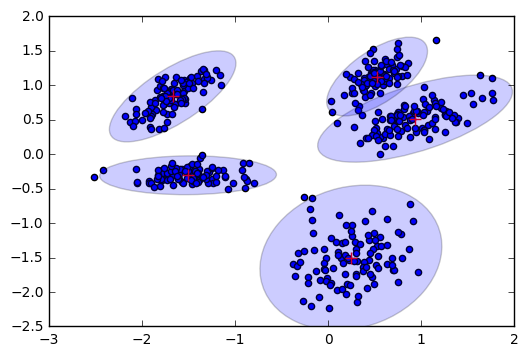
\includegraphics[scale=0.17]{em4.png}
  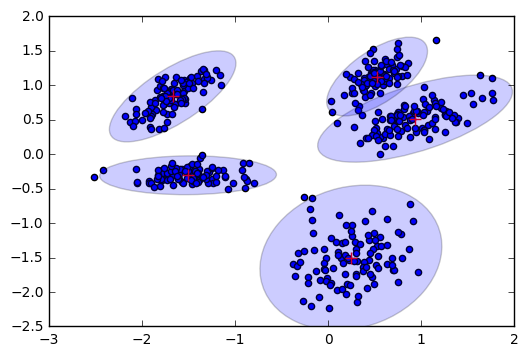
\includegraphics[scale=0.17]{em5.png}
  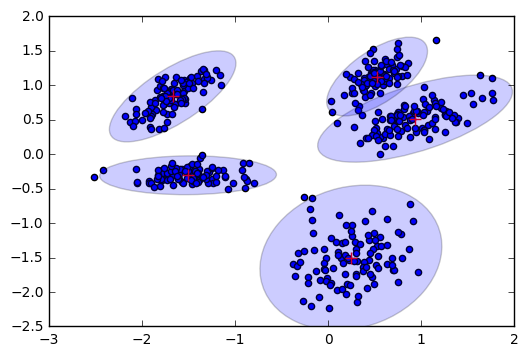
\includegraphics[scale=0.17]{em6.png}
  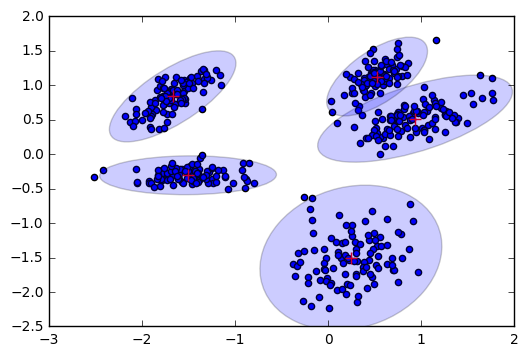
\includegraphics[scale=0.17]{em7.png}
  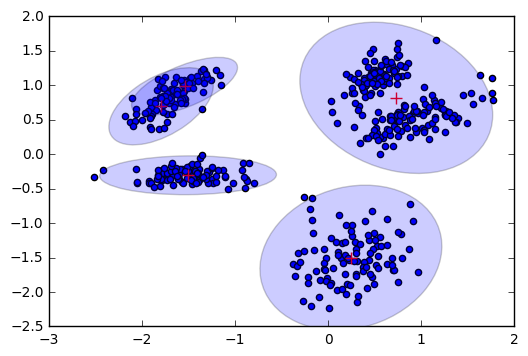
\includegraphics[scale=0.17]{em8.png}
  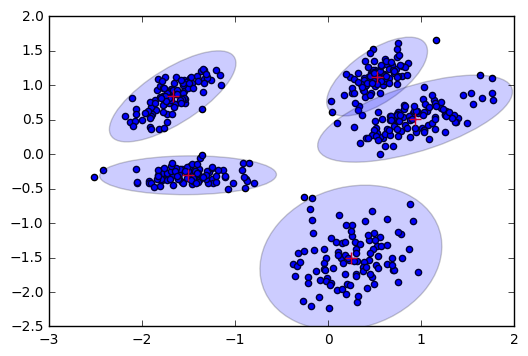
\includegraphics[scale=0.17]{em9.png}
  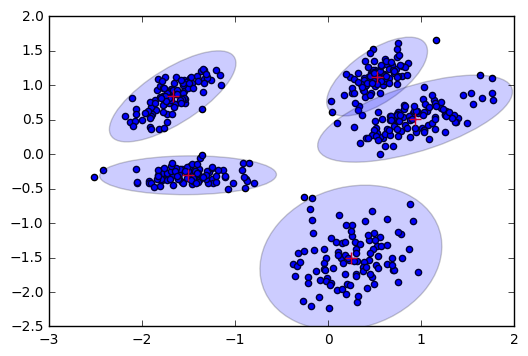
\includegraphics[scale=0.17]{em10.png}
  \caption{10 times plot with k=5 by GMM}
\end{figure}

\begin{verbatim}








\end{verbatim}

\subsection*{3.The initialisation of the GMM with a K-means}

\begin{figure}[htbp]
  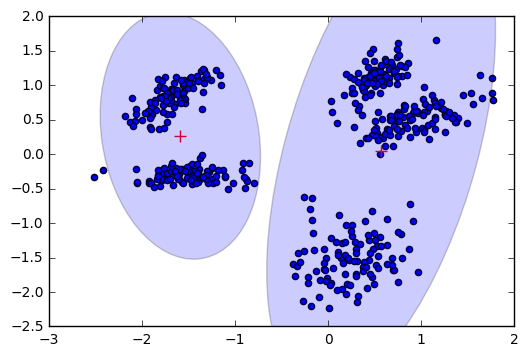
\includegraphics[scale=0.3]{gmmnkmk2.png}
  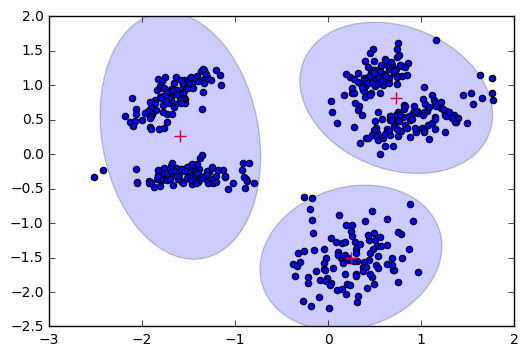
\includegraphics[scale=0.3]{gmmnkmk3.png}
  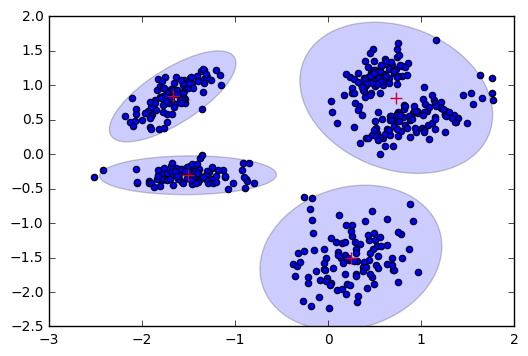
\includegraphics[scale=0.3]{gmmnkmk4.png}
  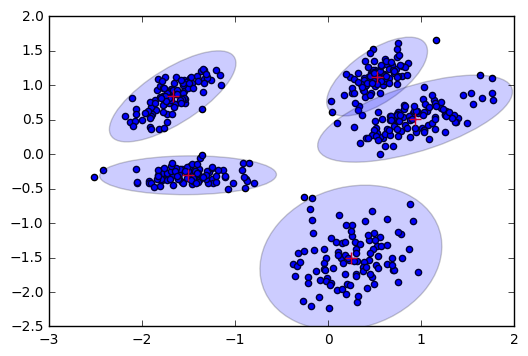
\includegraphics[scale=0.3]{gmmnkmk5.png}
  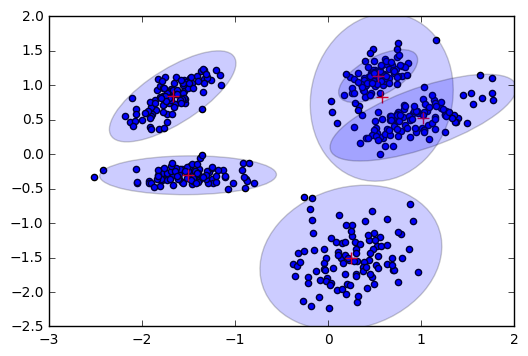
\includegraphics[scale=0.3]{gmmnkmk6.png}
  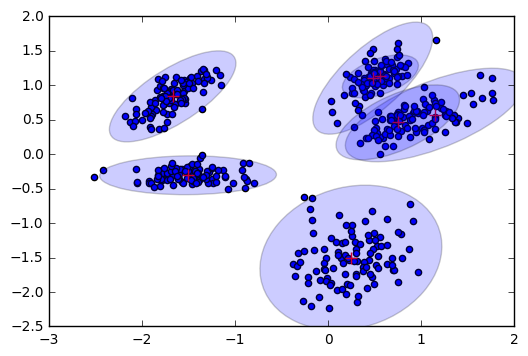
\includegraphics[scale=0.3]{gmmnkmk7.png}
  \caption{Plots from k=2 to K=7 }
\end{figure}

Both case of initialisation with K-means and without K-means the plots are same as above. But iteration times are reduced with K-means initialisation when k is smaller than 5 and when k is 5 iteration time is more stable than without K-means initialisation. When k is bigger than 5 it is no difference between them. Specially when k=3 is, K-means initialisation reduces iteration step very much. And the quality of the solutions for k=2 to k=5 are more stable with k-means. The most Remarkable case was k=3.

\begin{figure}[htbp]
  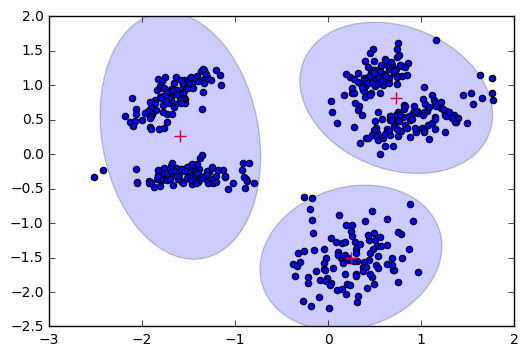
\includegraphics[scale=0.2]{k3nk1.png}
  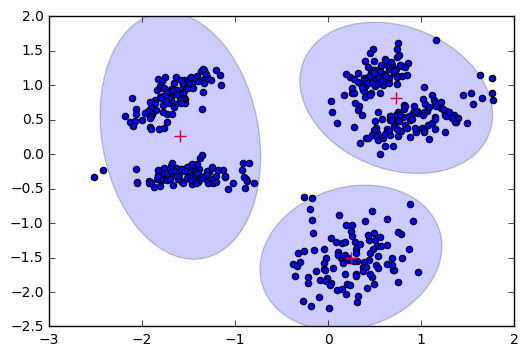
\includegraphics[scale=0.2]{k3nk2.png}
  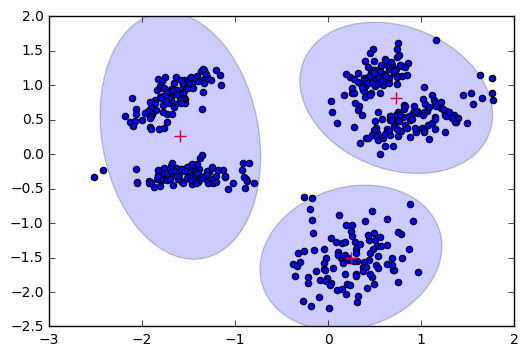
\includegraphics[scale=0.2]{k3nk3.png}
  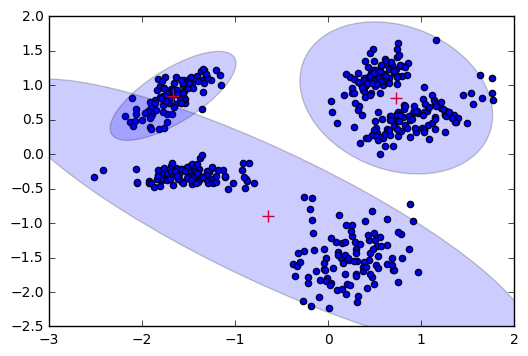
\includegraphics[scale=0.2]{k3nk4.png}
  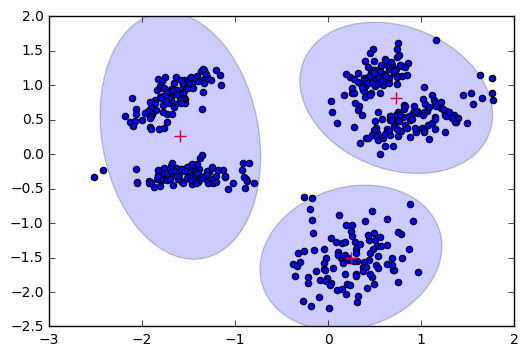
\includegraphics[scale=0.2]{k3nk5.png}
  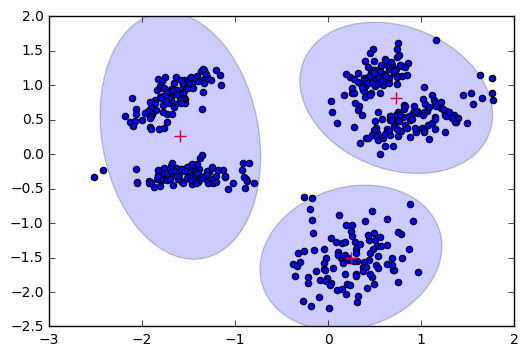
\includegraphics[scale=0.2]{k3nk6.png}
  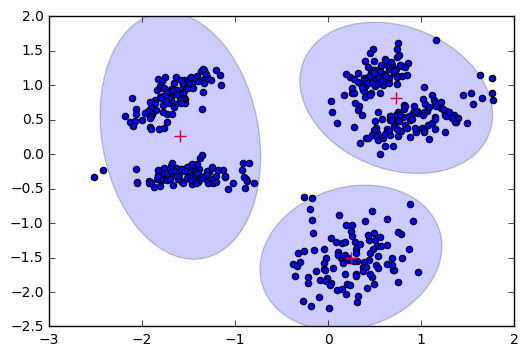
\includegraphics[scale=0.2]{k3nk7.png}
  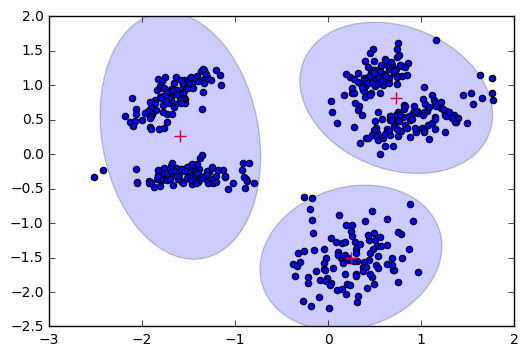
\includegraphics[scale=0.2]{k3nk8.png}
  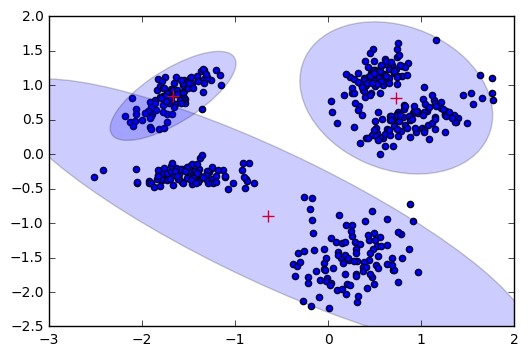
\includegraphics[scale=0.2]{k3nk9.png}
  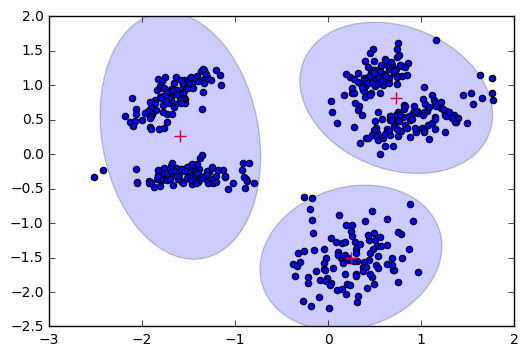
\includegraphics[scale=0.2]{k3nk10.png}
  \caption{10 Plots k=3 without K-means initialisation }
\end{figure}

\begin{figure}[htbp]
  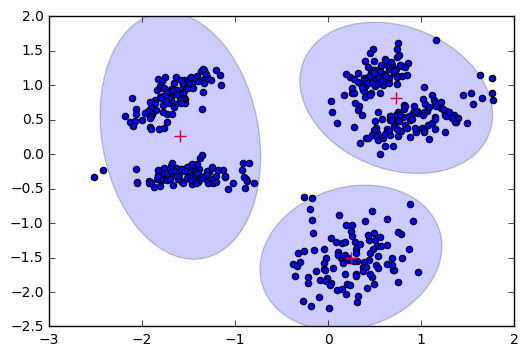
\includegraphics[scale=0.2]{k3wk1.png}
  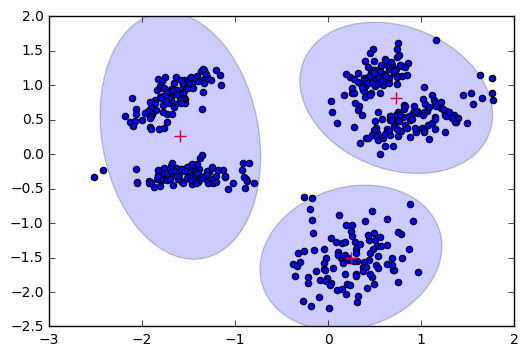
\includegraphics[scale=0.2]{k3wk2.png}
  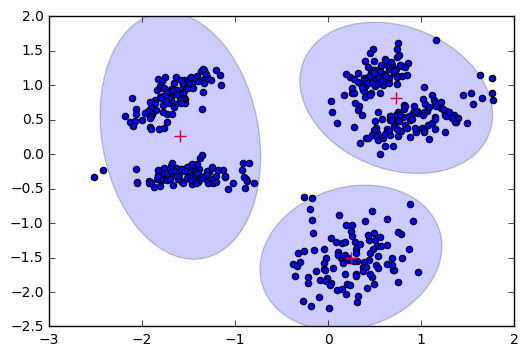
\includegraphics[scale=0.2]{k3wk3.png}
  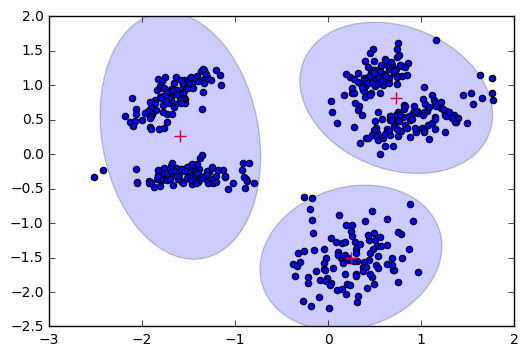
\includegraphics[scale=0.2]{k3wk4.png}
  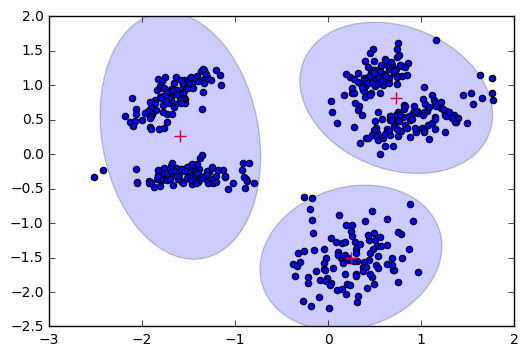
\includegraphics[scale=0.2]{k3wk5.png}
  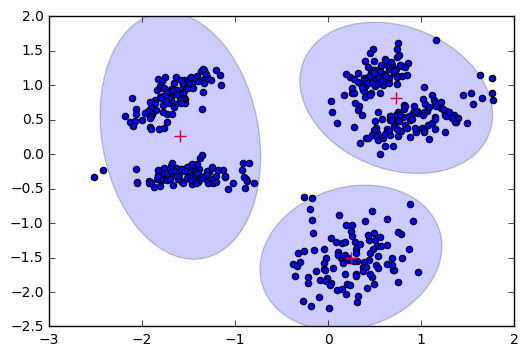
\includegraphics[scale=0.2]{k3wk6.png}
  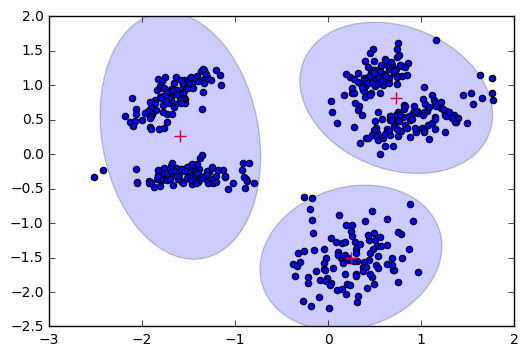
\includegraphics[scale=0.2]{k3wk7.png}
  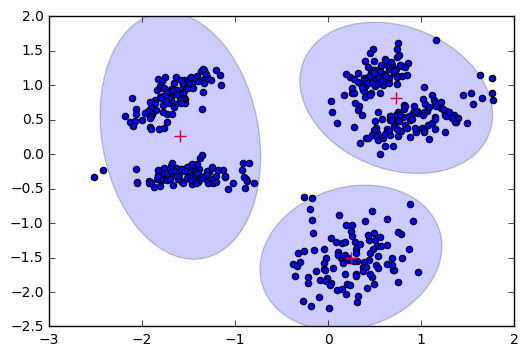
\includegraphics[scale=0.2]{k3wk8.png}
  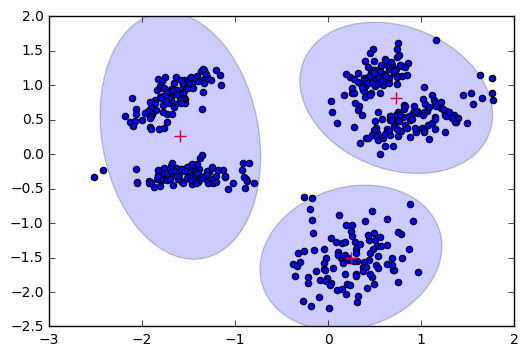
\includegraphics[scale=0.2]{k3wk9.png}
  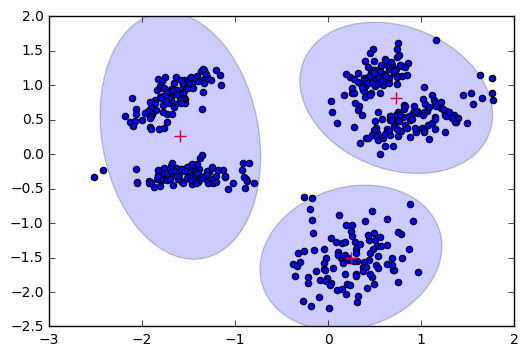
\includegraphics[scale=0.2]{k3wk10.png}
  \caption{10 Plots k=3 with K-means initialisation }
\end{figure}

\begin{verbatim}



\end{verbatim}

After plotting 10 times for k=3 with K-means initialisation and without it, there was 2 of 10 times false clustering in case without K-means but there was no false clustering with K-means initialisation. Therefore we can say that the quality of the solution with K-means is better than without.
The number of necessary iterations at each trial and averages of it are following.

\begin{verbatim}
Number of iterations without K-means: 27, 9, 23, 37, 20, 25, 5, 6, 19, 20
Average: 19.1
							  
Number of iterations with K-means: 7, 7, 7, 7, 7, 7, 6, 7, 7, 7
Average: 6.9
\end{verbatim}

The number of iterations are also much fewer and more stable with k-means than without. So k-means initialisation helps a lot to converge.

But why is it so remarkable when k=3 is? When we clusterise with 3 clusters every cluster will have similar variances in all directions. If we see one of this plot, we will find 5 concentrated datesets. 4 of them which are showed in upper left and upper right have deviated varianced so that the variances are high in x-axis and low in y-axis. But when we use three clusters, these datasets will be merged and the variances will be changed to be equaly in each direction. Because of equality of variances K-means becomes to work well. Therefore K-means initialisation works very well for k=3.


\begin{verbatim}


\end{verbatim}

\subsection*{4.Dendrogramm of the hierarchical clustering and a suitable value of k}

\begin{figure}[htbp]
  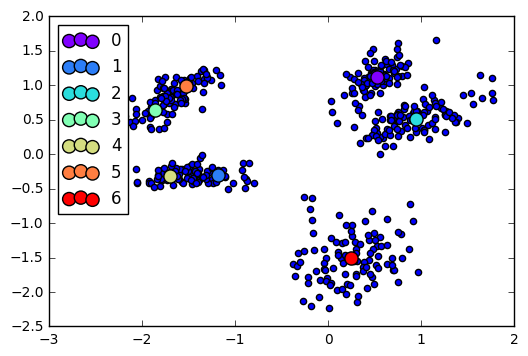
\includegraphics[scale=0.5]{kmfordend.png}
  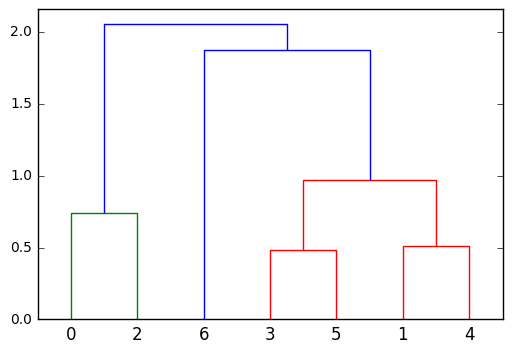
\includegraphics[scale=0.5]{dendg.png}
  \caption{K-means and the dendgram of the hierarchical clustering}
\end{figure}

The dendrogram shows that the loss of second merge doesn't increase much from the first merge.    But since the third merge the loss increases much before. Therefore it seems possible to pick a suitable value of k from this dendrogramm by setting a threshold for increasing value of loss. And loss value increase is over the threshold the merging should be stopped.Then we can get the suitable value of k=5. But the configuration of threshold is not easy.

\begin{figure}[htbp]
  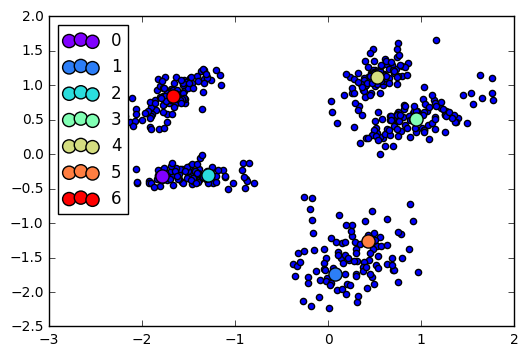
\includegraphics[scale=0.5]{kmfordend2.png}
  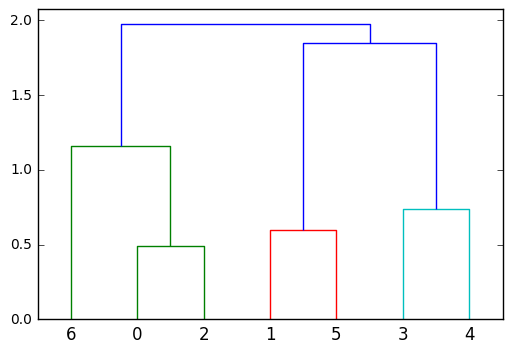
\includegraphics[scale=0.5]{dendg2.png}
  \caption{K-means and the dendgram of the hierarchical clustering}
\end{figure}

In this case the increasing loss value from the second mergin to third mergin is also same as from first to second. But from third to 4th the loss value changes much. Therefore if we use threshold in this case, we will get k=4 instead of k=5.
In my opinion sometimes we can get a a suitable value of k but dendrogram is not enough method to find it.

\section*{Assignment 8}

\subsection*{1.K-means and GMM for two deviated varianced gaussian dataset}

\begin{figure}[htbp]
 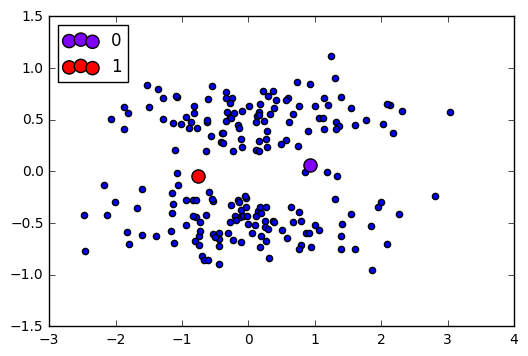
\includegraphics[scale=0.5]{km2gau.png}
 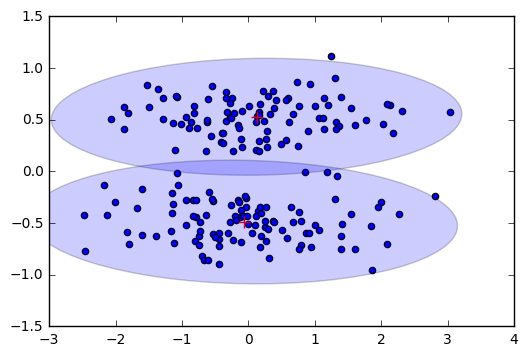
\includegraphics[scale=0.5]{em2gau.png}
 \caption{K-means and GMM}
\end{figure}
The graph shows clearly that GMM works better than K-means algorithm. The reason of this is that GMM estimate mean and covariance instead of simply finding k nearst neighbors.
By k-means algorithmu just nearest k neighbors are found. This means that this methos is based on a condition of same variance for all directions. The dataset "2gaussians" has high variance in x-axis but low direction in y-axis. Because of that when a neighbor is choosen, we must choose more neibors in x-axis but less neighbors in y-axis. But k-means can not choose depend on variance. On the other hands GMM choose them depend on variances.

\subsection*{2.}

\begin{verbatim}



\end{verbatim}


\section*{Assignment 9}

\subsection*{1. The cluster centers of USPS}

USPS is the matrix with (256x2007, dimension x num of data). At first we have to reduce the dimension to plot in 2D space. Then we use PCA.

\begin{verbatim}
X = usps['data_patterns']
pca=imp1.PCA(X.T)
Z =pca.project(X.T,2)
plt.scatter(Z[:,0],Z[:,1] )
\end{verbatim}

\begin{figure}[htbp]
  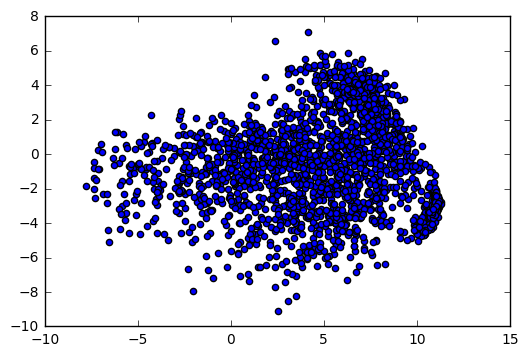
\includegraphics[scale=0.6]{pca.png}
  \caption{Projected in 2D space by PCA}
\end{figure}

And clustering by K-means

\begin{figure}[htbp]
  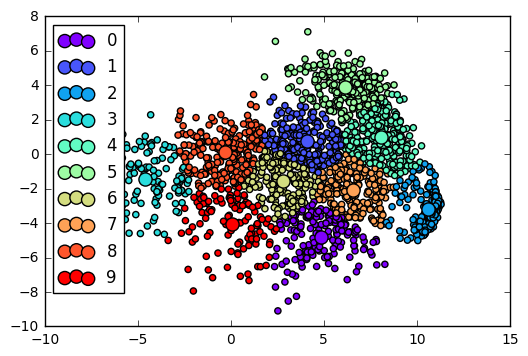
\includegraphics[scale=0.6]{uspskm.png}
  \caption{K-means clustering with USPS}
\end{figure}

And clustering by GMM

\begin{figure}[htbp]
  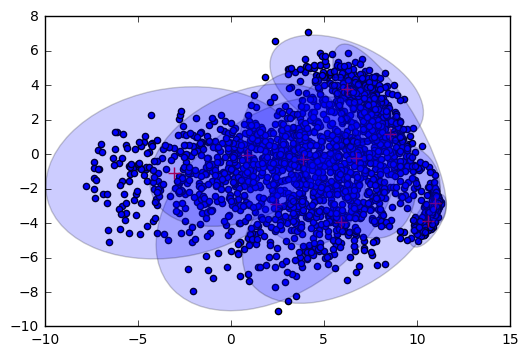
\includegraphics[scale=0.6]{uspsgmm.png}
  \caption{GMM clustering with USPS}
\end{figure}

\end{document}

